\begin{figure*}[t!hpb]
\caption{The LLOD Cloud}\label{f1}
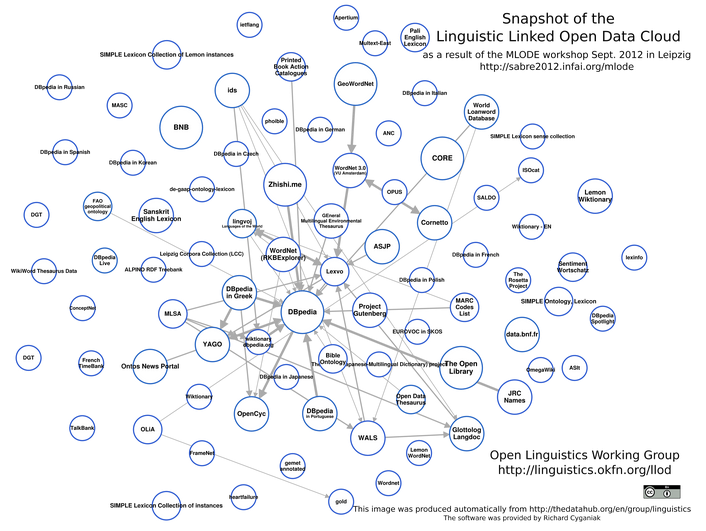
\includegraphics[width=15cm,keepaspectratio]{llod.png}
\end{figure*}

The Linguistics Linked Open Data cloud represents a portion of the Semantic Web network, and is specifically a sub cloud of the Linked Open Data cloud. It is maintained by the Open Linguistics Working Group\footnote{\url{http://linguistics.okfn.org/}}, which has three main goals for promoting openness in Linguistics: \begin{enumerate} \item Promoting the idea of open linguistic resources; \item Developing the means for the representation of open data; \item Encouraging the exchange of ideas across different disciplines. \end{enumerate}

Building an interoperable, linked data cloud is directly in line with these aims. The Open Knowledge Foundation, the umbrella organisation for the OWLG and other working groups, defines `openness' as "A piece of content or data [that] is open if anyone is free to use, reuse, and redistribute it -- subject only, at most, to the requirement to attribute and share-alike."\footnote{\url{http://opendefinition.org}} With this in mind, different databases within the Linked Open Data cloud have been marked out for inclusion within the LLOD. A diagram for the LLOD, developed by Cyganiak and Jentzsch, can be found at \url{http://lod-cloud.net} - this diagram is displayed in Fig. \ref{f1}. 

The following criteria must be met for a new linguistic resource to be included in the LLOD cloud: \begin{enumerate}\item The data is resolvable through HTTP, \item it is provided as RDF, \item it contains links to another data set in the diagram, and \item the entire data set must be available.\end{enumerate}. At the time of writing, the LLOD has {\it draft} status, meaning that several of the resources may point only to resource metadata, although each has been promised to be uploaded and linked to the LLOD in the near future. There are already many resources within the cloud, however, such as DBpedia, different RDF versions of WordNet, Cornetto (Dutch WordNet), OpenCyc, and the Open Data Thesaurus, metadata repositories like Lexvo and lingvoj. GOLD and ISOcat are currently available, although their license conditions are yet to be clarified. 


